
\section{Model}

\subsubsection*{Model introduction}
We consider a food-chain in a water column, consisting of a resource $R$ with concentration, a consumer $C$, and a predator $P$. The resource is thought of as phytoplankton, the consumer as copepods and the predator as forage fish. The predators and consumers are each distributed in the water column according to probability distributions, $\phi_c,\phi_p$, and the resource is distributed according to $r(z,t)$. See \Cref{fig:model_sketch}
\begin{figure}
 \begin{centering}
   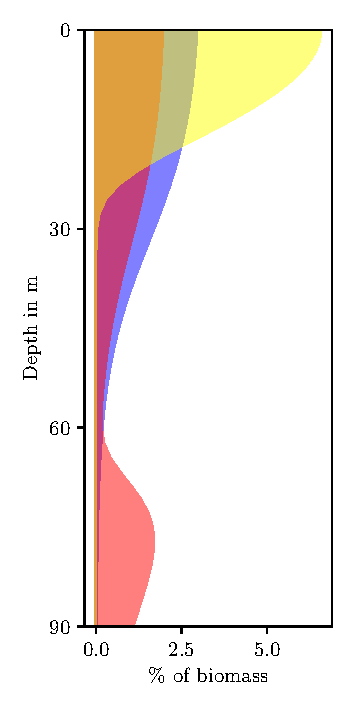
\includegraphics{plots/sketch_for_article.pdf}
 \end{centering}
 \label{fig:model_sketch}
 \caption{Sketch of model ecosystem, showing example distribution of resources, $(r(z,t)/R(t)$ \emph{(yellow)}, consumers ,$\phi_c$ \emph{(blue)} and predators, $\phi_p$ \emph{(red)}}
\end{figure}

Forage fish are visual predators, so their predation success is heavily light dependent. The available light decreases with depth in the water column, and varies with the time of day.
The light intensity $I$ at depth $z$ is approximately $I(z) = I_0\exp(-kz)$, and the light-dependent clearance rate of a predator is $\beta_{p,0}$.  However, even when there is no light available there is still a chance of catching a consumer if it is directly encountered,  so the clearance rate, $\beta_p(z,t)$, of forage fish never goes to 0 even at the middle of the night or at the deepest depths.
\begin{align*}
  \beta_p(z,t) = \beta_{p,0} \frac{I(z,t)}{1+I(z,t)} + \beta_{p,min}
\end{align*}


We model the light-levels at the surface via. the python package pvlib, using a simple Clear Sky model in Oresund between Denmark and Sweden. The light levels are given by the direct horizontal light intensity at the sea-surface, neglecting more complicated optic effects. The model takes the precitibale water $w_a$, and aerosol optical depth, $aod$. We model light decay throughout the water column as $\exp(-kz)$.


In contrast to forage fish, copepods are olfactory predators, and their clearance rate, $\beta_c$, is essentially independent of depth and light levels.
\begin{align*}
	\beta_c(z,t) &=  \beta_{c,0}
\end{align*}

The interactions between the consumer and resource are local, as are the interactions between a predator and a consumer. The local encounter rate between consumers and resources is given by $\beta_c(z,t)c(z,t)r(z,t)$, and the local encounter rate between predators and consumers is $\beta_p(z,t)c(z,t)p(z,t)$.

\subsubsection*{Population dynamics}

%Lotka-Volterra:
%\begin{align}
%  \label{eq:population_growth}
%  \dot{r} &= r(z,t)\pa{1-\frac{r(z,t)}{r_{max}(z)}} - \beta_c(z,t)c(z,t) r(z,t) + k \partial_x^2 r(z,t) \\
%  \dot{C} &=  \int_0^{z_0} \varepsilon \beta_c(z,t)c(z,t)r(z,t) dz- \int_0^{z_0} \beta_p(z,t) c(z,t) p(z,t) dz - C(t)\mu_C  %\\
%  \dot{P} &=  \int_0^{z_0} \varepsilon \beta_p(z,t) c(z,t)p(z,t) dz - P(t)\mu_P
%\end{align}
%The concentration of consumers, respectively predators is naturally given by a product of a probability density  $\phi_i,~i\in \{c,p\}$, describing the location in the water column and the total amount of consumers, respectively predators.
%\begin{align}
%	c(z,t) &= C(t)\phi_c(t, z) \\
%	p(z,t) &= P(t)\phi_p(t, z)
%  \label{eq:prob_dens}
%
%\end{align}
The resource cannot move actively, so its time dynamics are naturally specified locally. The growth of the resource is modeled with a logistic growth, with a loss from grazing by consumers and diffusion from the natural movement of the water. To simplify the model, we assume interactions can be described with a Type I functional response. %In natural environments, undersaturation of nutrients is the norm, \citep{}.


The total population growth of the consumer population is found by integrating the local grazing rate over the entire water column multiplied by a conversion efficiency $\epsilon$, subtracting the loss from predation. The growth of the predators is given by the predation rate integrated over the water column:
%Incorporating \Cref{eq:prob_dens} in \Cref{eq:population_growth}, we arrive at equations for the population dynamics governed by probability densities:
\begin{align}
	\dot{r} &= r(z,t)\pa{1-\frac{r(z,t)}{r_{max}(z)}} - \beta_c(z,t)\phi_c(z,t)C(t) r(z,t)  + k \partial_x^2 r(z,t)\\
	\dot{C} &= C(t)\left ( \int_0^{z_0} \varepsilon \beta_c(z,t)\phi_c(z,t)r(z,t) dz- P(t)\int_0^{z_0} \beta_p(z,t) \phi_c(z,t) \phi_p(z,t) dz - \mu_C \right ) \\
	\dot{P} &= P(t) \left ( C(t )\int_0^{z_0} \varepsilon \beta_p(z,t) \phi_c(z,t)\phi_p(z,t) dz - \mu_P \right )
  \label{eq:population_growth_prob_dens}
\end{align}


\subsubsection*{Fitness proxies and optimal strategies}


The instantaneous fitness pr. capita of a forage fish $(F_p)$ or copepod $(F_c)$ is given by the total growth divided by the biomass. We arrive at the fitness by dividing the population growth rate \Cref{eq:population_growth_prob_dens} by the total populations, eliminating the terms $C(t), P(t)$ outside the parantheses in \Cref{eq:population_growth_prob_dens}.

\begin{align}
	F_c(\phi_c, \phi_p) &= \int_0^{z_0} \varepsilon \beta_c(z,t)\phi_c(z,t)r(z,t) dz\\ &- P(t)\int_0^{z_0} \beta_p(z,t) \phi_c(z,t) \phi_p(z,t)dz \\
	F_p(\phi_c, \phi_p) &=  C(t) \int_0^{z_0} \varepsilon \beta_p(z,t)\phi_c(z,t)\phi_p(z,t) dz
  \label{eq:fitness}
\end{align}

At any instant, an organism seeks to find the strategy that maximizes its fitness. A strategy in our case is a probability distribution in the water column. The optimal strategy $\phi_c^*$ of a consumer depends on the strategy of the predators, and likewise for $\phi_p^*$ for the predators. Denoting the space of probability distributions on $[0,z_0]$ by $\mathbb{P}(0,z_0)$, this can be expressed as:
\begin{align*}
	\phi_c^*(z,t)(\phi_p) &= \argmax_{\phi_c \in \mathbb{P}(0,z_0)}  \int_0^{z_0} \varepsilon \beta_c(z,t)\phi_c(z,t)r(z,t) dz \\ &- P(t)\int_0^{z_0} \beta_p(z,t) \phi_c(z,t) \phi_p(z,t)dz  \\
	\phi_p^*(z,t)(\phi_c) &= \argmax_{\phi_p \in \mathbb{P}(0,z_0)}C(t) \int_0^{z_0} \varepsilon \beta_p(z,t)\phi_c(z,t)\phi_p(z,t) dz
\end{align*}

Consumers and predators maximize their fitness simultaneously, leading to a \emph{Nash Equilibrium}, where neither can gain anythin from diverging from their strategy. The Nash equilibrium of the instantaneous game is:
\begin{align}
  \label{eq:nash_equilibria}
	\phi_c^{*,NE} &=  \argmax_{\phi_c \in P(0,z_0)}  \int_0^{z_0} \varepsilon \beta_c(z,t)\phi_c(z,t)r(z,t) dz \\ &- P(t)\int_0^{z_0} \beta_p(z,t) \phi_c(z,t) \phi_p^{*,NE}(z,t) dz \\
	\phi_p^{*,NE} &=  \argmax_{\phi_p \in P(0,z_0)}C(t) \int_0^{z_0} \varepsilon \beta_p(z,t)\phi_c^{*,NE} \phi_p(z,t) dz
\end{align}

\subsubsection*{Noisy strategies} %	Y \sim \mathcal{N}(0, \sigma^2) \\
Our model incorporates that fish are not necessarily perfectly rational, but have \textbf{bounded rationality} by letting the strategy depend on the rationality parameter $\sigma$, with $\sigma=0$ being completely rational and $\sigma = \infty$ completely irrational. Rather than choosing a precise location, an individual can choose where it diffuses around. As fish cannot swim out of the top of the ocean, nor through the bottom, we end with the partial differential equation:
\begin{align}
  \label{eq:density_PDE}
	&\partial_\sigma \phi_i = \partial_z^2 \phi_i \\
	&\partial_z \phi_i \mid_{z=0} = 0 \\
  &\partial_z \phi_i \mid_{z = z_0} = 0
\end{align}
The equation \Cref{eq:density_PDE} has the fundamental solution $f_Y(\sigma)$, determined by the method of images. Instead of choosing a distribution $\phi$, an individual chooses a distribution $f_X$, which we use as initial condition in \Cref{eq:density_PDE}. An individual with strategy $f_X$ will actually be distributed according to $\phi(\sigma,z)$, which becomes increasingly uniform as $\sigma$ increases. The way we concretely solve \Cref{eq:density_PDEs} with initial condition $f_X$ is through a Greens function approach, ie. performing a convolution of $f_X$ and $f_Y$. We refer to the solution $\phi$ of \Cref{eq:density_PDE} as the realized distribution.

We expect that an individual will still attempt to maximize its own fitness, even though the location cannot be chosen exactly. Instead, the optimization will go towards finding the strategy $f_X$ that maximizes the fitness when noise is taken into account.
Having introduced noise to the strategies of consumers and predators, we can find the Nash equilibrium of their optimal distributions without noise. We find the Nash pair by inserting the fundamental solution in \Cref{eq:nash_equilibria} and optimizing over $f_{X_i},~i\in \{c, p\}$.
\begin{align*}
	f_{X_c}^{*,NE} &=  \argmax_{f_{X_c} \in \mathbb{P}(0,z_0)}  \int_0^{z_0} \varepsilon \beta_c(z,t)(f_{X_c} * f_Y) r(z,t) dz \\ & -  P(t)\int_0^{z_0} \beta_p(z,t) (f_{X_c} * f_Y)(f_{X_p}^{*,NE} * f_Y) dz \\
	f_{X_p}^{*,NE} &=  \argmax_{f_{X_p} \in \mathbb{P}(0,z_0)}C(t) \int_0^{z_0} \varepsilon \beta_p(z,t)(f_{X_c}^{*,NE}  * f_Y)(f_{X_p}* f_Y) dz
\end{align*}

The realized distributions are found by convolution with $f_Y$ as
\begin{align*}
  \phi_c^{*,NE} &= f_{X_c}^{*,NE} * f_Y \\
  \phi_p^{*,NE} &= f_{X_p}^{*,NE} * f_Y
\end{align*}

\subsubsection*{Spatial discretization}
We discretize the interval $[0,z_0]$ with a spectral scheme based on Legendre polynomials, \citep{kopriva2009implementing}, which allows precise integration and differentation with only relatively few points.
We approximate pure strategy of being in a point $z_i$  by a normalized hat-function $e_i$, zero everywhere apart from $z_i$.
\begin{align*}
	& \int_{z_i}^{z_{i+1}} e_i dz = 1 \\
	&e_i(z_{i-1}) = 0,~ e_i(z_{i+1}) = 0
\end{align*}
Working on a grid with $N$ points, a strategy chosen by a consumer or predator then becomes a linear combination of hat-functions,
\begin{align*}
  &\phi_{i} = \sum_{j<N} a_{j,i} e_j, \quad i\in \{c,p\} \\
  &\sum_{j<N} a_{j,i} = 1 \quad i\in \{c,p\}
\end{align*}
The strategy of a player is fully determined by the $a_i$'s.

When considering non-optimal actors, we need to implement the convolution with $f_Y$, which also assures that the resulting distrbution is smooth. An added benefit of incorporating bounded rationality then becomes that our strategy profiles are guaranteed to be smooth, decreasing the number of points needed for exact evaluation of the integrals.


\subsubsection*{Finding the Nash Equilibrium and time-stepping}
Finding the Nash Equilibrium in a game in continuous space is usually a very hard task, requiring the development of bespoke methods, \citep{verticalmigration}, or very long runtimes, \citep{jerome}. The method we have use circumvents these problems, by combining a little-known result in mathematical optimization with a spectral scheme.

By discretizing space, we have reduced an uncountable strategy set to a more manageable finite amount, with pure strategies $e_i$. The gain of a consumer playing strategy $e_i$ against a predator playing strategy $e_j$ can be determined as $F_c(e_i,e_j)$, \Cref{eq:fitness}, and similarly for a predator. Both payoff functions are bi-linear in the strategies, which allows us to write up payoff matrices $E_c, E_p$, with entry $(i,j)$ determined through $F_k(e_i,e_j), k \in \{c, p\}$. If a predator plays strategy $s_p$, given by a vector $(a_1,\dots,a_N)$ and a consumer plays strategy $s_c$ given by $(b_1,\dots,b_N)$, the consumer and predator payoffs can be determined through $E_c,E_p$ as:
\begin{align*}
  F_c(s_c,s_p)&=\ip{s_c}{E_c s_p} \\
  F_p(s_c,s_p)&=\ip{s_p}{E_p s_p}
\end{align*}
Our discretization has reduced the problem to a bimatrix game, where finding the Nash equilibrium is more tractable. A bimatrix game is a special case of a polymatrix game, where $n$ players play against each other in pairwise games and the total payoff is given by the sum of the payoffs across the pairwise interactions.

It does not appear to have diffused through the literature, but the Nash equilibrium of a polymatrix game can be found by solving a linear complementarity problem \citep{miller1991copositive}. Therefore our approach provides an avenue to reduce the intractable problem of finding a Nash equilibrium of a multiplayer game in continuous space to solving an optimization problem.
When solving the linear complementarity problem, the first step is to introduce the total payoff matrix:
\begin{align*}
	R_{init} = \begin{bmatrix} 0 & E_c \\ E_p & 0 \end{bmatrix}
\end{align*}
As all entries in $R_{init}$ do not have the same sign, $R_{init}$ is not copositive. We fix this by defining $R=R_{init}-max(R_{init})$.
Applying the results of \citep{miller1991copositive}, to find the Nash equilibrium we need to solve the problem:
\begin{align}
	(Hz+q) = w & \\
	\ip{z}{w} = 0 & \\
	z\geq 0, w\geq 0
  \label{eq:lcp}
\end{align}
where
\begin{align*}
  H &= \begin{bmatrix} -R & -A^T \\ A & 0 \end{bmatrix}
	A &= \begin{bmatrix} -1 &-1 & \dots & -1 \\  -1 &-1 & \dots & -1 \end{bmatrix} \\
	q &= \begin{pmatrix} 0 &\dots & 0 & -1 & -1 \end{pmatrix}   \\
\end{align*}

Solving \Cref{eq:lcp} was done through two different methods. The interior-point method as implemented in IPOPT, \citep{wachter2006implementation}, called via. the auto-differentation software CasADi \citep{Andersson2019}, and Lemkes Algorithm implemented in the Numerics package in Siconos, \citep{acary2019introduction}. Experience showed that Lemkes algorithm was the fastest, but there is probably a situation where the problem has a sparsity structure favorable to IPOPT.

With a fast algorithm for finding the Nash Equilibrium in hand, we are able to solve the time-dynamics for the predator-prey system by a Euler-scheme. The dynamics of the resource are more complicated due to the diffusion term, \Cref{eq:population_growth_prob_dens}. We solve the partial differential equation for the resource using the method of exponential time-differencing with a first-order approximation of the integral. Using exponential time-differencing guarantees a stable solution, though the system may be stiff, \cite{hochbruck2010exponential}. %\subsubsection*{Time evolution}

%We solve the time-evolution of the predator and prey populations using a semi-implicit euler scheme. At each step we find the Nash equilibrium based on the last state, and evolve the populations accordingly. The time-evolution of the resource is solved by the method of exponential time differencing, using a first-order difference, \citep{hochbruck2010exponential}, ie. a mixture of a first-order method and an exact Greens function approach.

\subsubsection*{Model parametrization}
Following \citep{yodzis1991}, we parametrize the clearance and loss rates in a metabolically scaled manner following Kleibers law, \citep{kleiber}, using scaling constants from \citep{kha_2019}. We use the default parameters in the clear-sky model, modelling a sequence of moonless nights. This is a bit of a simplification, but it should not have a great effect on our results. The North Sea is modeled with a rather high attenueation coefficient.


\begin{tabular}{l | l | l}
  Precipitable water & $w_a$ & 1 g $\cdot$ m$^{-3}$\\
  Aeorosol optical depth & $aod$ & 0.1 \\
  Light decay & $k$ & 0.1 m$^{-1}$\\
  Ocean depth & $z_0$ & 90 m \\
  Consumer mass & $m_c$ & 0.05 $g$ \\
  Predator mass & $m_p$ & 20 $g$ \\
  Consumer clearance rate & $\beta_c$ & 32 m$^{3}$ year$^{-1}$ \\
  Predator clearance rate & $\beta_p$ & 2800 m$^3$ year$^{-1}$ \\
  Consumer metabolic rate & $\mu_c$ & 0.24 g$^{3}$ year$^{-1}$ \\
  Predator metabolic rate & $\mu_p$ & 21 g$^3$ year$^{-1}$ \\
  Minimal attack rate & $\beta_0$ & $5 \cdot 10^{-3} \beta_p$ \\
  Phytoplankton growth & $\lambda$ & 100 year$^{-1}$ \\
  Phytoplankton max & $r_{max}$ & $10\mathcal{N}(0,6)$ g$\cdot$m$^{-1}$ \\
  Irrationality & $\sigma$ & 14 $m^2$ \\
  Diffusion rate & k & 500 m$^{2}$ year$^{-1}$
\end{tabular}
